% !TEX root = /Users/Gela/Desktop/Thesis_latex/thesis.tex


\section{Flowchart investigation}
Two different setups for a comparing system to the current system were investigated, section \ref{Flowchart}, and one system, System 2 were chosen to be the comparing system. Both Systems were considered fulfilling most of the requirements, section \ref{framing}, for an updated version. Restrictions on the membrane, such as requirements on no back pressure on the membrane lead to the decision on chosing System 2 as a comparing system. 

The two comparing systems were set to:\\
\begin{figure}[h]
\centering
\begin{minipage}{.5\textwidth}
    \centering
    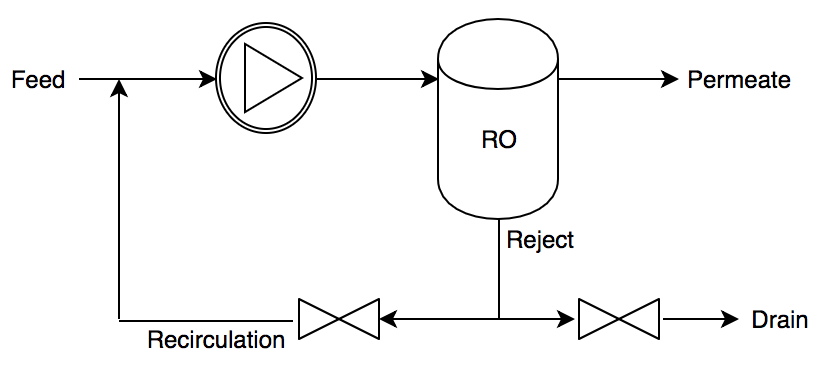
\includegraphics[width=0.8\textwidth]{Sys1}
    \caption{Current System}
    \label{fig:System1}
\end{minipage}%
\begin{minipage}{.5\textwidth}
  \centering
  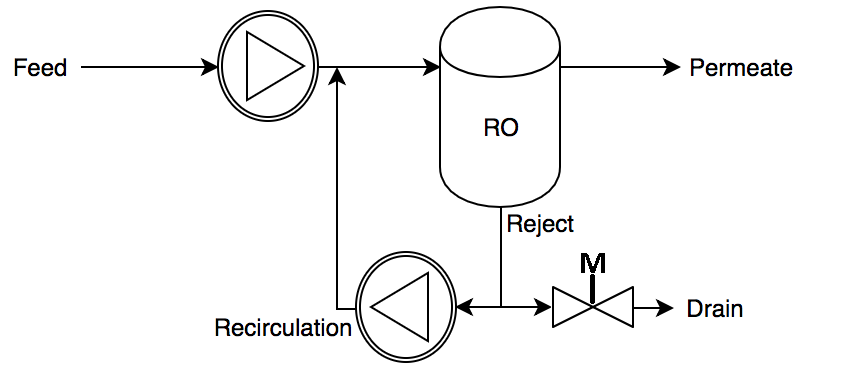
\includegraphics[width=.8\linewidth]{Sys2}
  \caption{System 2}
  \label{fig:System2}
\end{minipage}
\end{figure}

\section{Tests}
\subsection{Current system}
Results for the test on the current system, figure \ref{fig:Sys1}:

PLOTS FIGURES DATA

\subsection{System 2}


\section{Modeling}
A physical model of the membrane were made and the given results can be seen in: 

\section{Implementation Test Rig}


\subsection{Connections}
In Figure (\ref{fig:PressConn}-\ref{fig:PumpConn}) all connections in the test rig is displayed.


\begin{figure}[h]
    \centering
    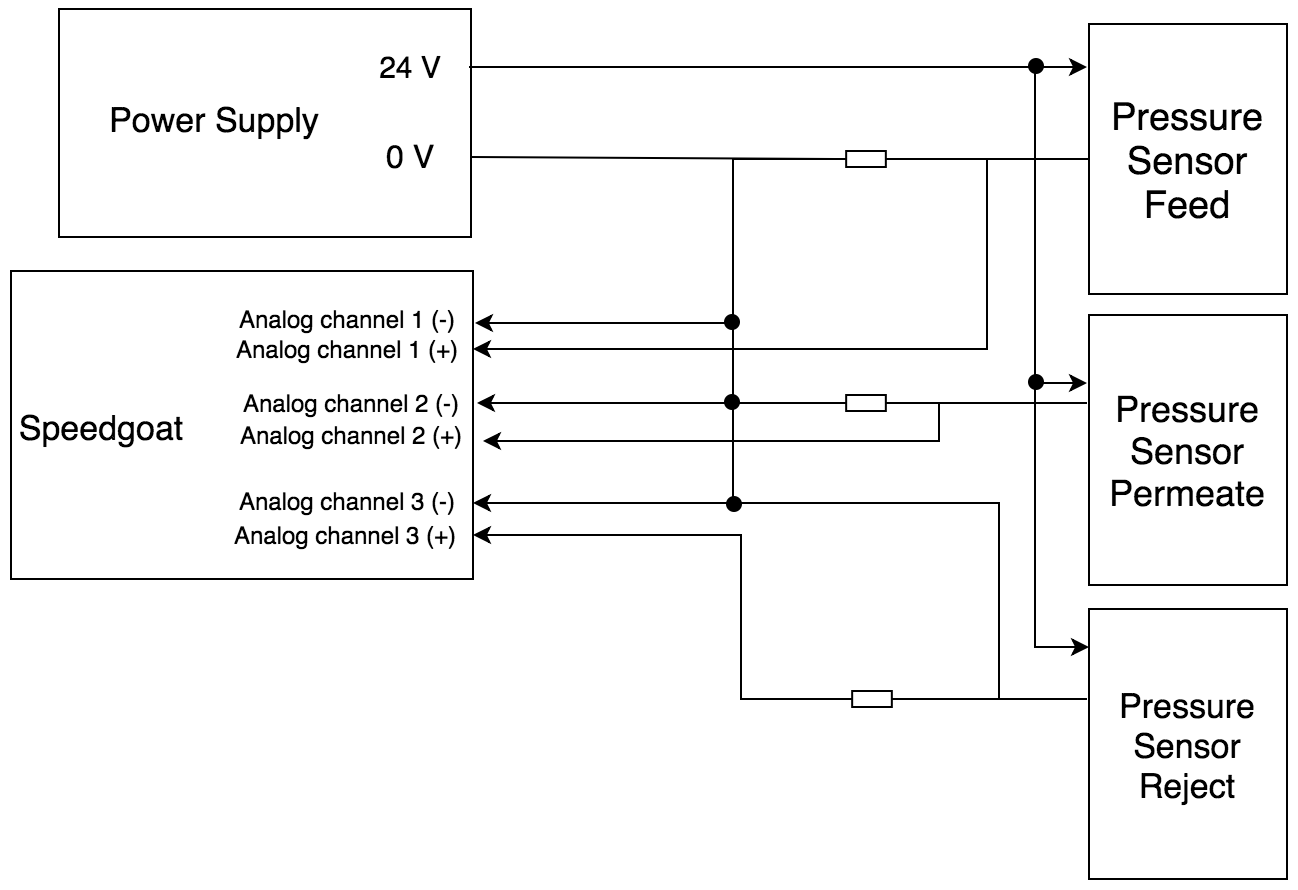
\includegraphics[width=0.7\textwidth]{PressConn}
    \caption{Connections Pressure sensors}
    \label{fig:PressConn}
\end{figure}

\begin{figure}[h]
    \centering
    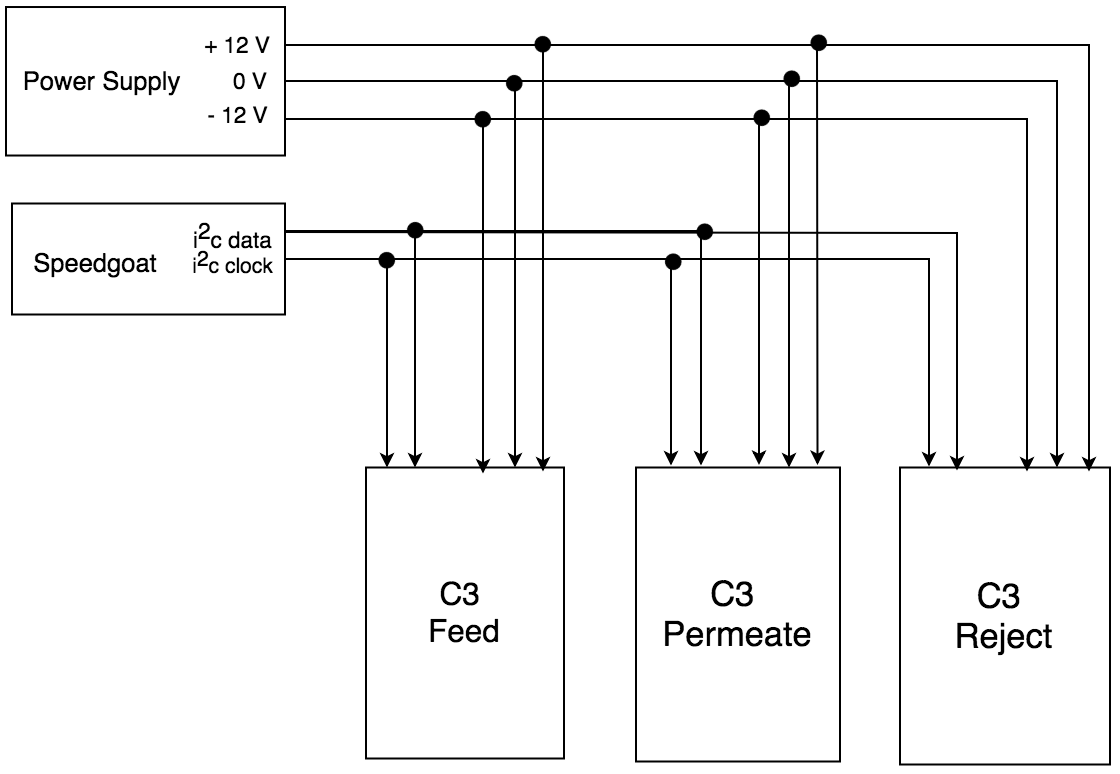
\includegraphics[width=0.7\textwidth]{C3Conn}
    \caption{Connections measurement blocks, C3}
    \label{fig:C3Conn}
\end{figure}

\begin{figure}[h]
    \centering
    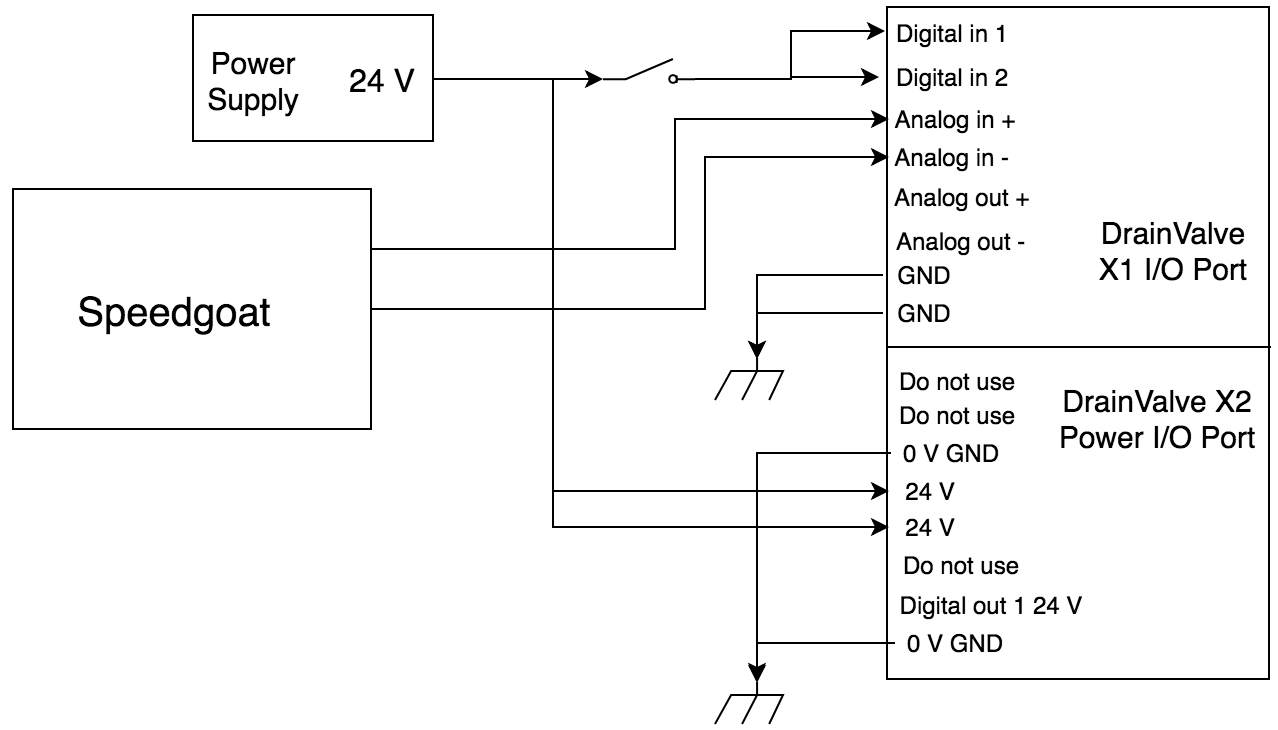
\includegraphics[width=0.7\textwidth]{ValveConn}
    \caption{Connections Drain Valve}
    \label{fig:ValveConn}
\end{figure}

\begin{figure}[h]
    \centering
    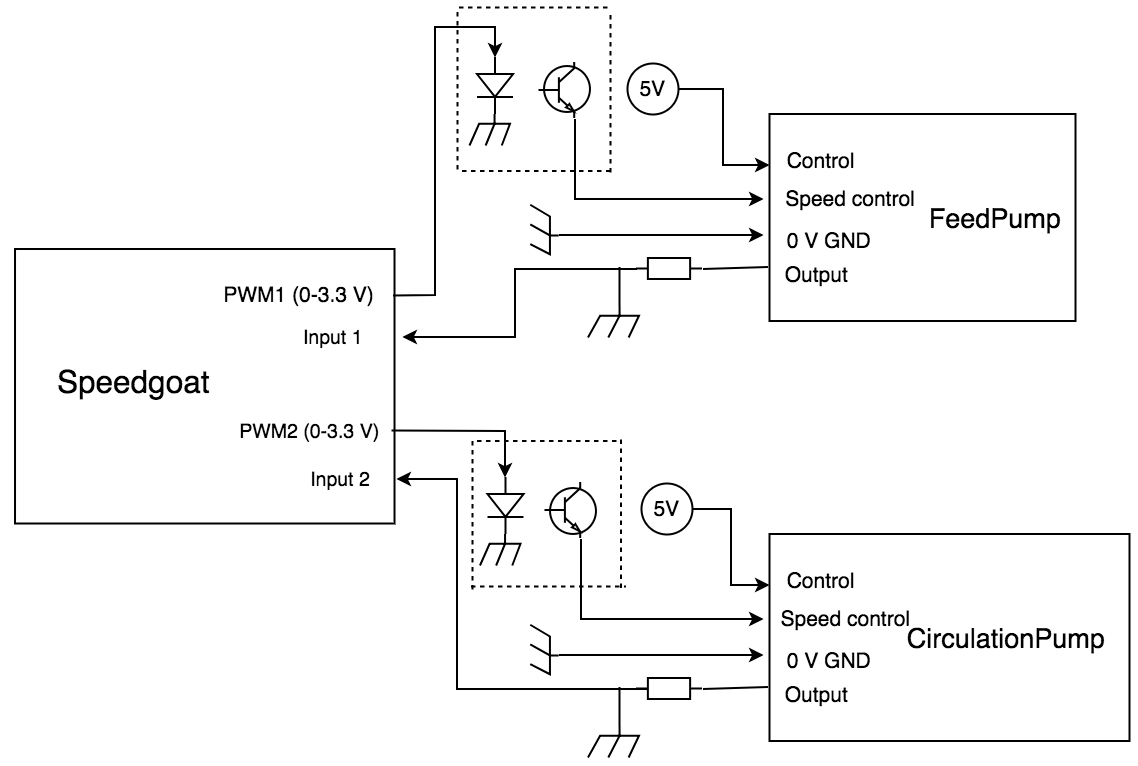
\includegraphics[width=0.7\textwidth]{PumpConn}
    \caption{Connections pumps}
    \label{fig:PumpConn}
\end{figure}


\section{Mapping}
\begin{figure}[h]
    \centering
    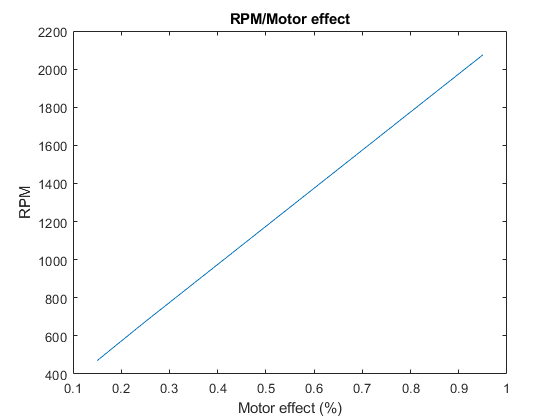
\includegraphics[width=0.7\textwidth]{RPM.png}
    \caption{RPM Pumps}
    \label{fig:RPM}
\end{figure}


\begin{figure}[h]
    \centering
    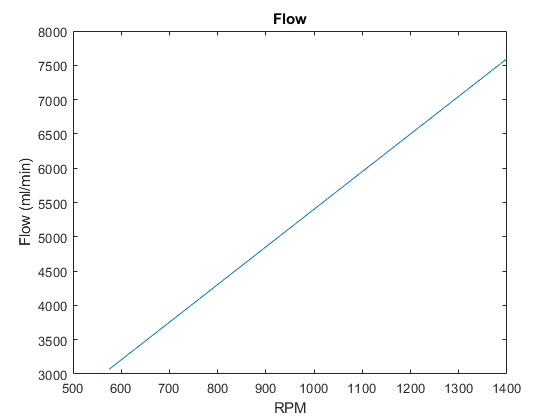
\includegraphics[width=0.7\textwidth]{Flow.png}
    \caption{Flowrate}
    \label{fig:Flowrate}
\end{figure}


\section{Design of control algorithms}

\begin{figure}[h]
    \centering
    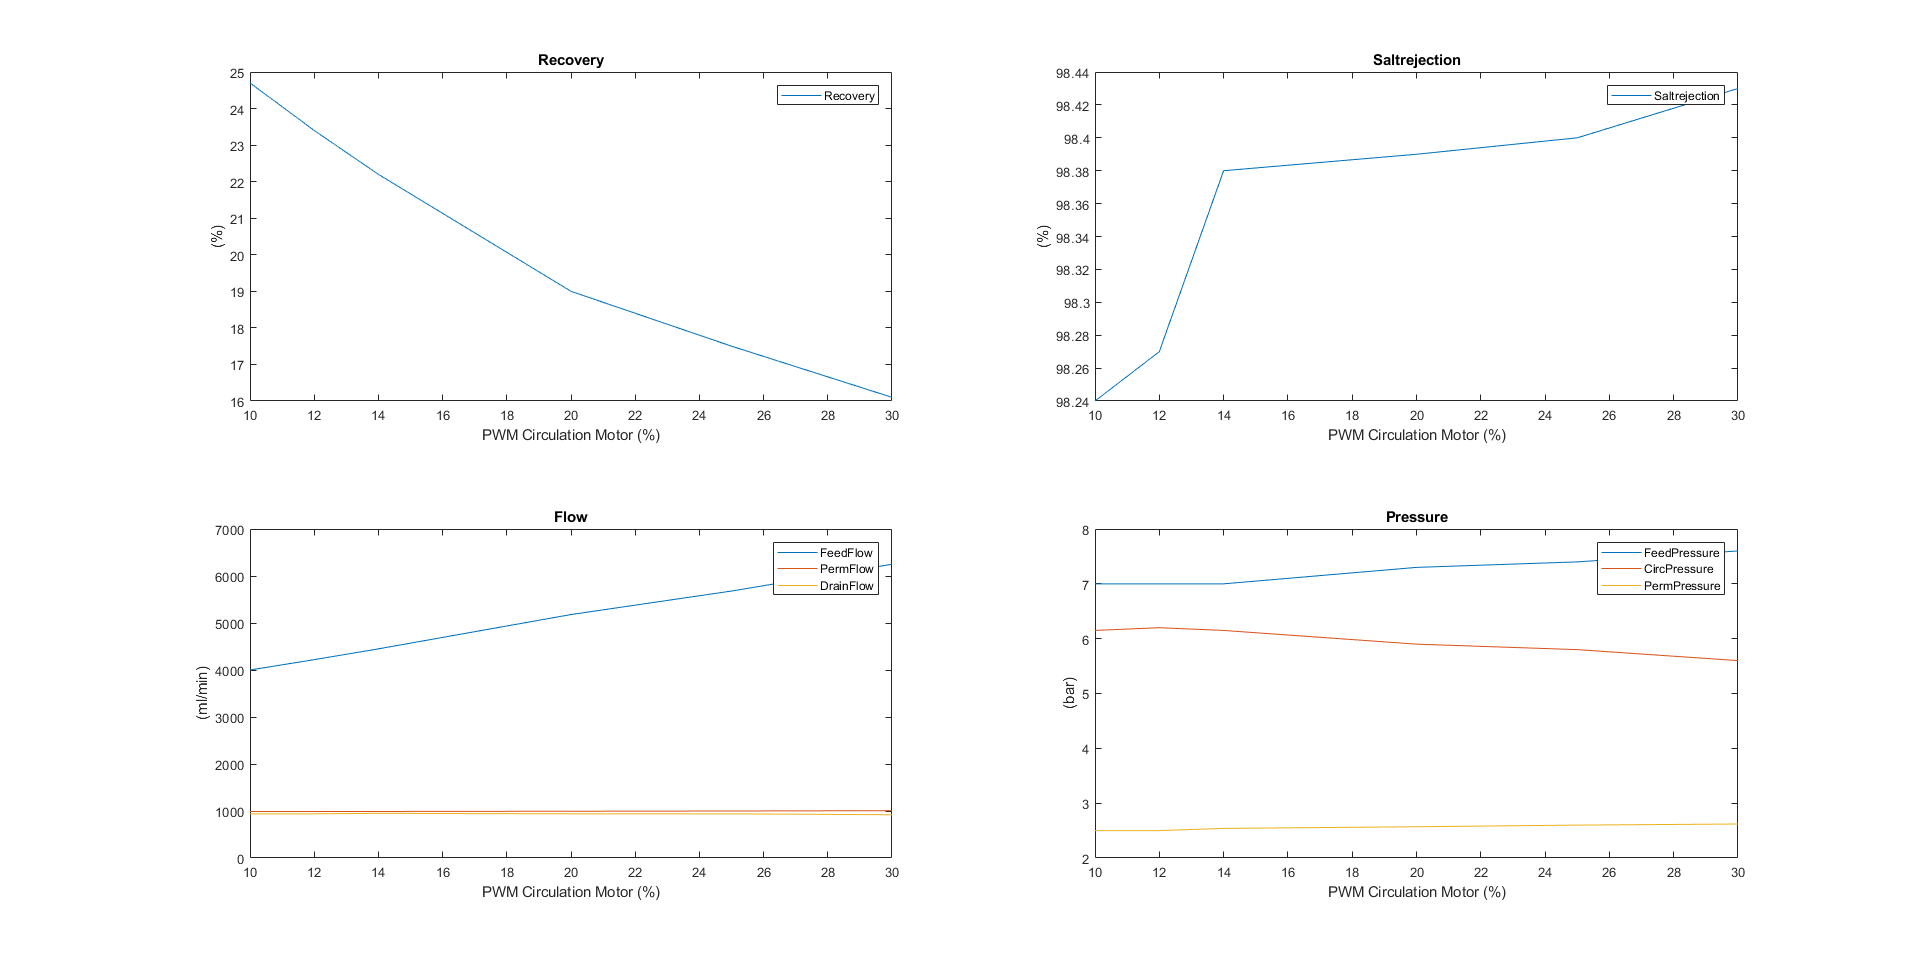
\includegraphics[width=1.65\textwidth, angle = 270]{PreTestReg1.png}
    \caption{Tests with recycle pump as changing parameter}
    \label{fig:PreTestReg1}
\end{figure}

\begin{figure}[h]
    \centering 
    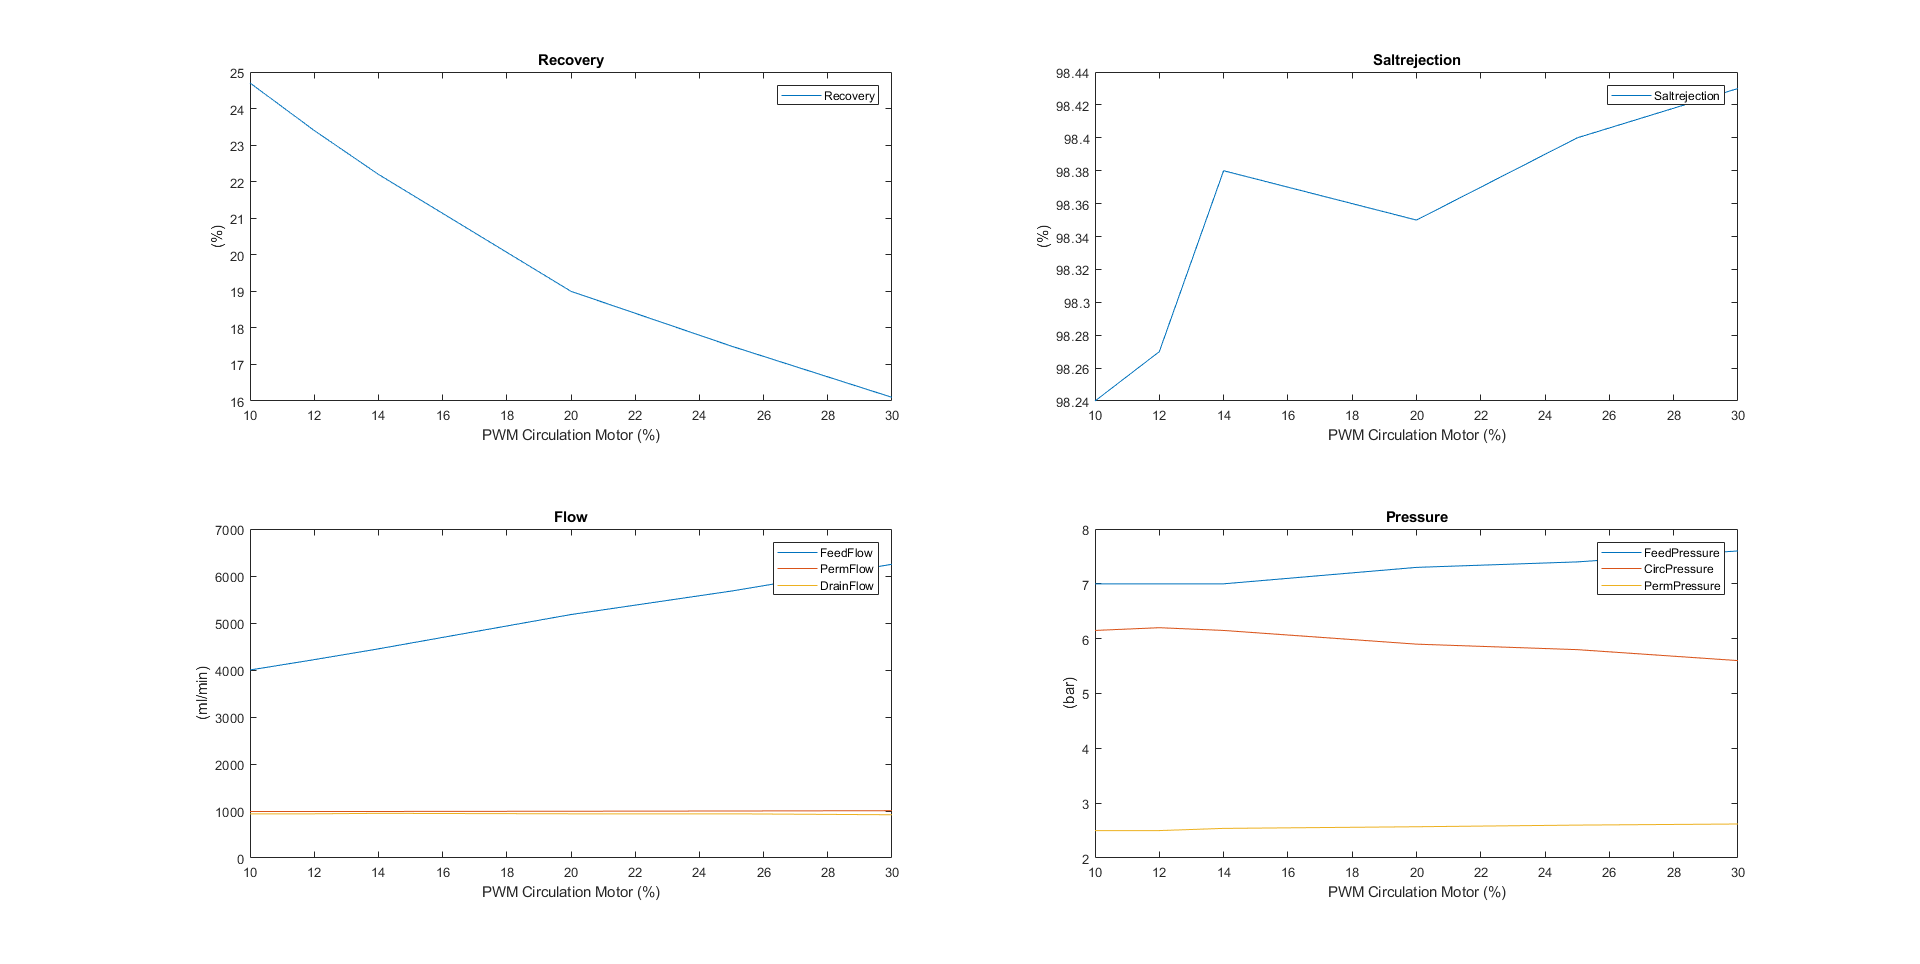
\includegraphics[width=1.65\textwidth, angle=270]{PreTestReg3.png}
    \caption{Tests with inlet pump as changing parameter}
    \label{fig:PreTestReg3}
\end{figure}





FIGURES AND PLOTS FROM SIMSCAPE


\section{Control simulations}




\section{Improvements}
